\def\regenfigs{0}
\documentclass[anonymous,sigconf,9pt]{acmart}

\usepackage{microtype}
\if\regenfigs1
\usepackage{tikz,pgfplots}
\usetikzlibrary{arrows.meta}
\usepgfplotslibrary{groupplots}
\usepgfplotslibrary{external}
\usepgfplotslibrary{colorbrewer}
\pgfplotsset{cycle list/Set1}
\usepgfplotslibrary{fillbetween}
\pgfplotsset{compat=1.18}
\pgfplotsset{
    tick align=outside,
    tick pos=left,
    xmajorgrids,
    x grid style={white},
    ymajorgrids,
    y grid style={white},
    axis line style={white},
    axis background/.style={fill=white!89.803921568627459!black},
    legend style={draw=none, fill=none},
    legend cell align=left,
}
\pgfkeys{/pgf/number format/.cd, 1000 sep={\,}}

\pgfplotsset{
    log x ticks with fixed point/.style={
        xticklabel={
            \pgfkeys{/pgf/fpu=true}
            \pgfmathparse{2^\tick}%
            \pgfmathprintnumber[fixed relative, precision=4]{\pgfmathresult}
            \pgfkeys{/pgf/fpu=false}
        }
    },
    log10 x ticks with fixed point/.style={
        xticklabel={
            \pgfkeys{/pgf/fpu=true}
            \pgfmathparse{10^\tick}%
            \pgfmathprintnumber[fixed relative, precision=3]{\pgfmathresult}
            \pgfkeys{/pgf/fpu=false}
        }
    },
    log y ticks with fixed point/.style={
        yticklabel={
            \pgfkeys{/pgf/fpu=true}
            \pgfmathparse{2^\tick}%
            \pgfmathprintnumber[fixed relative, precision=4]{\pgfmathresult}
            \pgfkeys{/pgf/fpu=false}
        }
    }
}
\fi

\begin{figure}[tbp]
    \centering
    %\includegraphics[width=\linewidth]{results//cache-carveout-h100-hbm3/h100_carveout_placeholder.png}
\if\regenfigs1
\begin{tikzpicture}
\begin{axis}[
    thick,
    %xmode=log,
    %ymode=log,
    legend style={at={(1.0,0.25)},anchor=east},
    xlabel={Shared memory carveout [KiB]},
    title={Perf. relative to ``default'' carveout},
    height=2in,
    ymin=-0.05,
    width=\linewidth,
]
    \addplot+[mark=*] table[y index=1] {results/cache-carveout-h100-hbm3/carveout_data_h100_hbm3_new.txt};
    \addlegendentry{ComputeUi};
    \addplot+[mark=square*] table[y index=2] {results/cache-carveout-h100-hbm3/carveout_data_h100_hbm3_new.txt};
    \addlegendentry{ComputeYi};
    \addplot+[mark=diamond*] table[y index=3] {results/cache-carveout-h100-hbm3/carveout_data_h100_hbm3_new.txt};
    \addlegendentry{ComputeFusedDeidrjAll};
    \addplot+[mark=triangle*] table[y index=4] {results/cache-carveout-h100-hbm3/carveout_data_h100_hbm3_new.txt};
    \addlegendentry{PairComputeLJCut};
\end{axis}
\end{tikzpicture}
\else
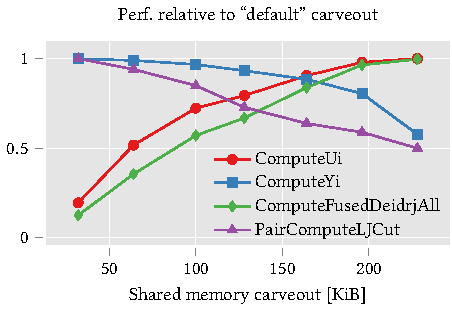
\includegraphics{generated-figures/paper-figure3.pdf}
\fi
    \caption{Performance of the \texttt{ComputeUi}, \texttt{ComputeYi}, and \texttt{ComputeFusedDeidrjAll} kernels in SNAP and the pairwise force kernel \texttt{PairComputeLJCut} in Lennard-Jones as a function of the shared memory carveout on NVIDIA H100-HBM3-SXM. The performance is normalized against the ``default'' value selected at runtime. All runs were at 1,024,000 atoms.}
    \label{fig:cache_carveout}
\end{figure}

\end{document}
 